\documentclass{article}
\usepackage{multicol}
\usepackage{listings}

\usepackage{xcolor}

\usepackage{graphicx}

 
\definecolor{codegreen}{rgb}{0,0.6,0}
\definecolor{codegray}{rgb}{0.5,0.5,0.5}
\definecolor{codepurple}{rgb}{0.58,0,0.82}
\definecolor{backcolour}{rgb}{0.95,0.95,0.92}
 
\lstdefinestyle{austyle}{
    backgroundcolor=\color{backcolour},   
    commentstyle=\color{codegreen},
    keywordstyle=\color{magenta},
    numberstyle=\tiny\color{codegray},
    stringstyle=\color{codepurple},
    basicstyle=\footnotesize,
    breakatwhitespace=true,         
    breaklines=true,                 
    captionpos=b,                    
    keepspaces=true,                 
    numbers=left,                    
    numbersep=5pt,                  
    showspaces=false,                
    showstringspaces=false,
    showtabs=true,                  
    tabsize=2,
    lineskip=4pt,
    numberblanklines=false
}
 
\lstset{style=austyle}

\usepackage[ampersand]{easylist}
\newenvironment{easyenum}{\begin{easylist}[enumerate]}{\end{easylist}}
\newenvironment{easyitem}{\begin{easylist}[itemize]}{\end{easylist}}

\usepackage{todonotes}

\newcommand{\openquestion}[1]{\bigskip\todo[inline, backgroundcolor=blue!20!white]{\textbf{Open question:} #1}\bigskip}

\newenvironment{modprovides}
{\medskip\par\noindent This module \emph{provides} the ability to:
\begin{easyitem}}
{\end{easyitem}}
\newenvironment{modrequires}
{\medskip\par\noindent This module \emph{requires} the ability to:
\begin{easyitem}}
{\end{easyitem}}

\newcommand{\itemtt}[1]{\item \texttt{#1}}

\title{Design Specifications for exaMPI\\ v0.1}
\author{Shane Farmer, Nawrin Sultana, Alexander Calvert\\Auburn Project Lead: Dr. Anthony Skjellum}

\begin{document}

\maketitle
\tableofcontents
 
\section{Language and Engineering}

The library will primarily be written in C++, with extensions TBD but likely at least C++11.  Template metaprogramming and other techniques will be used to optimize the code where such gains are reasonable; the Boost library will be avoided unless serious justifications (not yet provided) are made.

Standard project scaffolding will be provided in the form of Makefiles, READMEs, and so forth.

\section{Public Interface}

The publicly accessible interface provided by the library will be C-style and consist of the required subset of MPI as specified in the requirements document and expanded on below.  This C interface will pair with a backing C++ thin-layer implementation that dispatches the calls to the library internals.  The interface implementation itself will be modularized enough to allow for interface versioning, if\footnote{When.} it becomes necessary in the future.

\subsection{Identified Public MPI Calls Required}

\begin{lstlisting}[language=C]

/* Core MPI API */

int MPI_Abort(MPI_Comm, int)
int MPI_Allgather(void *, int, MPI_Datatype, void *, int, MPI_Datatype, MPI_Comm)
int MPI_Allreduce(void *, void *, int, MPI_Datatype, MPI_Op, MPI_Comm)
int MPI_Alltoall(void *, int, MPI_Datatype, void *, int, MPI_Datatype, MPI_Comm)
int MPI_Barrier(MPI_Comm)
int MPI_Bcast(void *, int, MPI_Datatype, int, MPI_Comm)
int MPI_Comm_create(MPI_Comm, MPI_Group, MPI_Comm *)
int MPI_Comm_create_group(MPI_Comm, MPI_Group, int, MPI_Comm *)
int MPI_Comm_rank(MPI_Comm, int *)
int MPI_Comm_size(MPI_Comm, int *)
int MPI_Comm_split(MPI_Comm, int, int, MPI_Comm *)
int MPI_Finalize(void)
int MPI_Gather(void *, int, MPI_Datatype, void *, int, MPI_Datatype, int, MPI_Comm)
int MPI_Group_create_session(MPI_Session, char *, MPI_Group *)
int MPI_Iallreduce(void *, void *, int, MPI_datatype, MPI_Op, MPI_Comm, MPI_Request *)
int MPI_Ibcast(void *, int, MPI_Datatype, int, MPI_Comm, MPI_Request *)
int MPI_Icheckpoint(MPI_Comm, MPI_Request *)
int MPI_Igather(void *, int, MPI_Datatype, void *, int, MPI_Datatype, int, MPI_Comm, MPI_Request *)
int MPI_Ireduce(void *, void *, int, MPI_Datatype, MPI_Op, int, MPI_Comm, MPI_Request *)
int MPI_Iscatter(void *, int, MPI_Datatype, void *, int, MPI_Datatype, int, MPI_Comm, MPI_Request *)
int MPI_Init(int *, char ***)
int MPI_Init_info(int *, char ***, MPI_Info)
int MPI_Irecv(void *, int, MPI_Datatype, int, int, MPI_Comm, MPI_Request *)
int MPI_Isend(void *, int, MPI_Datatype, int, int, MPI_Comm, MPI_Request *)
int MPI_Recv_init(void *, int, MPI_Datatype, int, int, MPI_Comm, MPI_Request *)
int MPI_Reduce(void *, void *, int, MPI_Datatype, MPI_Op, int, MPI_Comm)
int MPI_Scatter(void *, int, MPI_Datatype, void *, int, MPI_Datatype, int, MPI_Comm)
int MPI_Send_init(void *, int, MPI_Datatype, int, int, MPI_Comm, MPI_Request *)
int MPI_Session_get_names(MPI_Session, char **)
int MPI_Session_init(MPI_Info, MPI_Errhandler, MPI_Session *)
int MPI_Session_finalize(MPI_Session *)
int MPI_Start(MPI_Request *)
int MPI_Startall(int, MPI_Request *)
int MPI_Wait(MPI_Request *, MPI_Status *)
int MPI_Waitall(int, MPI_Request *, MPI_Status *)
int MPI_Wtime(void)
 
 
/* MPI Profiling API */
 
int PMPI_Abort(MPI_Comm, int)
int PMPI_Allgather(void *, int, MPI_Datatype, void *, int, MPI_Datatype, MPI_Comm)
int PMPI_Allreduce(void *, void *, int, MPI_Datatype, MPI_Op, MPI_Comm)
int PMPI_Alltoall(void *, int, MPI_Datatype, void *, int, MPI_Datatype, MPI_Comm)
int PMPI_Barrier(MPI_Comm)
int PMPI_Bcast(void *, int, MPI_Datatype, int, MPI_Comm)
int PMPI_Comm_create(MPI_Comm, MPI_Group, MPI_Comm *)
int PMPI_Comm_create_group(MPI_Comm, MPI_Group, int, MPI_Comm *)
int PMPI_Comm_rank(MPI_Comm, int *)
int PMPI_Comm_size(MPI_Comm, int *)
int PMPI_Comm_split(MPI_Comm, int, int, MPI_Comm *)
int PMPI_Finalize(void)
int PMPI_Gather(void *, int, MPI_Datatype, void *, int, MPI_Datatype, int, MPI_Comm)
int PMPI_Group_create_session(MPI_Session, char *, MPI_Group *)
int PMPI_Iallreduce(void *, void *, int, MPI_datatype, MPI_Op, MPI_Comm, MPI_Request *)
int PMPI_Ibcast(void *, int, MPI_Datatype, int, MPI_Comm, MPI_Request *)
int PMPI_Icheckpoint(MPI_Comm, MPI_Request *)
int PMPI_Igather(void *, int, MPI_Datatype, void *, int, MPI_Datatype, int, MPI_Comm, MPI_Request *)
int PMPI_Ireduce(void *, void *, int, MPI_Datatype, MPI_Op, int, MPI_Comm, MPI_Request *)
int PMPI_Iscatter(void *, int, MPI_Datatype, void *, int, MPI_Datatype, int, MPI_Comm, MPI_Request *)
int PMPI_Init(int *, char ***)
int PMPI_Init_info(int *, char ***, MPI_Info)
int PMPI_Irecv(void *, int, MPI_Datatype, int, int, MPI_Comm, MPI_Request *)
int MPI_Isend(void *, int, MPI_Datatype, int, int, MPI_Comm, MPI_Request *)
int PMPI_Recv_init(void *, int, MPI_Datatype, int, int, MPI_Comm, MPI_Request *)
int PMPI_Reduce(void *, void *, int, MPI_Datatype, MPI_Op, int, MPI_Comm)
int PMPI_Scatter(void *, int, MPI_Datatype, void *, int, MPI_Datatype, int, MPI_Comm)
int PMPI_Send_init(void *, int, MPI_Datatype, int, int, MPI_Comm, MPI_Request *)
int PMPI_Session_get_names(MPI_Session, char **)
int PMPI_Session_init(MPI_Info, MPI_Errhandler, MPI_Session *)
int PMPI_Session_finalize(MPI_Session *)
int PMPI_Start(MPI_Request *)
int PMPI_Startall(int, MPI_Request *)
int PMPI_Wait(MPI_Request *, MPI_Status *)
int PMPI_Waitall(int, MPI_Request *, MPI_Status *)
int PMPI_Wtime(void)

\end{lstlisting}

\section{Internal Interfaces and Modularization}

To address the flexibility requirement of the library, and to assist and enforce good design principles, the library is broken into several modules which may be altered at compile-time or runtime\footnote{This is subject to change}.  

Here, by ``module'' we mean an identifiable related set of code functionality that can be fulfilled by a unit of code conforming to a well-defined internal interface.  Properly designed, the modularization of the library will break it into pieces that isolate (and intelligently group) functionality while maintaining the semantic breadth required for performance.

These internal interfaces are driven by the various dependencies within the library proper.

\paragraph{Implementation} The specification of the modules\footnote{i.e. the interface} is provided as abstract base classes in C++\footnote{More specifically, classes consisting entirely of pure virtual functions.} which are in turn fulfilled by specific implementations of the modules.  Given a sensible design and interface conformance, the modules should recombine at will to provide specific functionality during runtime.

It is not necessarily our position or intent that multiple versions of each module will be provided in this research effort, but some modules are near-guaranteed to receive such treatment, and others provide interesting avenues for investigation.

\begin{figure}
	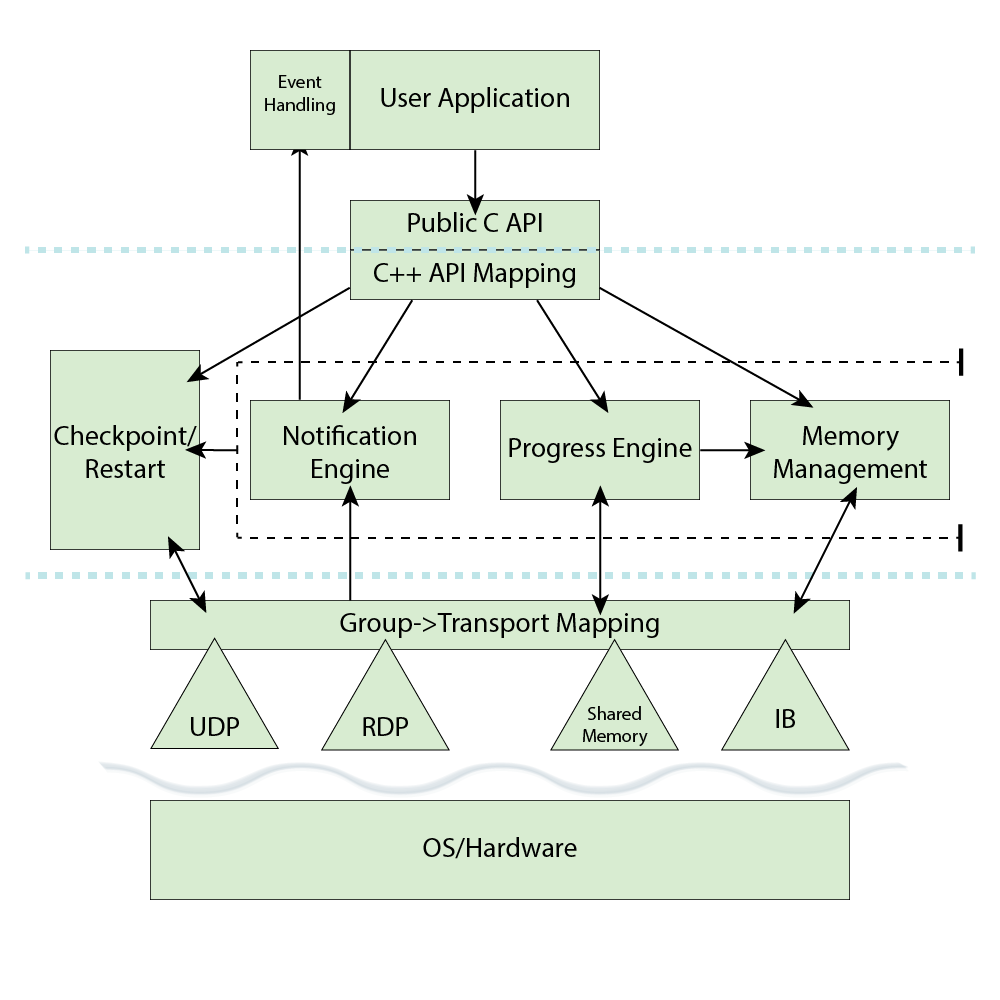
\includegraphics[width=\linewidth]{module}
	\caption{Module Structure}
	\label{fig:module}
\end{figure}
We provide the module types below.

\subsection{Interface}

As mentioned above, the public interface itself will need code to translate the C-style public calls to internal C++ calls.  This layer provides that semantic with the minimum logic necessary to translate the requests to the appropriate layers.

\begin{modprovides}
& Invoke the C-style calls comprising the public MPI API
& Request specific versions of the interface
\end{modprovides}

\begin{modrequires}
& Initiate send and receive requests
& Query notifications
& Establish custom data types
\end{modrequires}

\subsubsection{Calls}

The calls provided by the Interface module are expected to be entirely application-facing; no calls are provided for library internals.  Therefore, the calls provided consist exactly of the public API.\footnote{Even where we in the future implement interface version requesting, that will function as an extension of the \emph{public} API.}



\subsection{Progress}

The progress engine is a core piece of MPI and has deep effects on performance characteristics.  We here isolate it\footnote{As much as possible, anyway; the progress engine, as might be expected, has deep ties to the overall function of the library.} to allow for various implementations and experimentation.

\paragraph{Event Queues}  Notification of completion\footnote{Including error cases.} is a fundamental role of an asynchronous system, required here.  A callback system has simpler semantics and implementation than a proper event queue, but has limitations w/r/t thread affinity and core usage in concurrent systems.  We therefore fix the progress engine interface as providing a full-fledged event queue with poll-like alternative semantics.

\begin{modprovides}
& Queue messages for sending
& Queue buffers for receiving
& Request notifications through an event queue
& Manage, donate, initiate, affine, and/or schedule system threads
\end{modprovides}

\begin{modrequires}
& Set up a network send through a transport
& Set up a network receive through a transport
& Translate an MPI rank to a specific address through a transport
& Evaluate network statistics and characteristics
& Validate provided buffers as ready for transfer
\end{modrequires}


\subsection{Memory}

The memory module exists in recognition of the various requirements placed on memory by the combination of MPI semantics and the variety of transports available to HPC applications.  Those functions requiring buffer management are isolated here to avoid unnecessary reimplementation of memory pools, pinning caches, and so forth.

\begin{modprovides}
& Manage memory pools in both raw and transport-ready states
& Track and/or provide user buffers in light of the above
& Manage semantics and provide characteristics of user data types
\end{modprovides}

\begin{modrequires}
& Validate a buffer as transport-ready
\end{modrequires}

\openquestion{Should the memory module provide shared memory semantics for on-node communication between MPI processes?  A first analysis suggests these transactions are simply messages across a different type of transport, but is there room for enhancement if we instead treat them as a special type of memory buffer?}



\subsection{Transport}

The transport modules are responsible for providing a meaningful interface with common semantics that maintains optimizations.\footnote{Of all the goals of the project, this familiar one is the most difficult, and likely impossible to achieve without some form of compromise.  For that reason, the transport interface should be viewed as having the highest risk of instability.}  Because a system may wish to utilize multiple transports (and by necessity if shared memory is implemented as a transport) there is a need to support multiple loaded transports simultaneously; modularization makes this fairly straightforward but introduces a requirement for some care in the semantics.

\openquestion{Is it worth the semantic overhead of adding another module to represent a \emph{group} of transports?  SF: my opinion here is that we could easily implement a group transport as a transport itself and keep logic for distribution there, but this merits some discussion, IMO.}

\openquestion{How best to handle addresses, and in what module do the various responsibilities live?  It's nontrivial to divorce the requirements, since the progress engine will likely need some notion of locality when considering ranks, and will need to maintain some type of mapping between ranks and the specific transports that understand their addresses; a full-traversal approach through transport modules may fail due to ambiguous addresses (consider TCP vs. IPoIB).}

\begin{modprovides}
& Send and receive buffers across the network
& Do some form of address resolution and/or mapping
& Track status of outstanding network requests
& Cleanly initialize, bind, and destroy network instances
& Query requirements (and fulfillment) of buffers for network transport
\end{modprovides}




\subsection{Fault}

We propose a fault detection module, which takes over the responsibilities of fault validation to the extent that can be divorced from other modules.

\openquestion{\emph{Can} these responsibilities be divorced?  What functionality is required of this module to validate existing data, communications, and transactions?  SF:  This may map to extensions to the public API, but it's hard to figure out how this could operate without requiring hooks inside the other modules, which would require special flavors of those and call into question the need for this module.  However, there is definitely recovery logic that could live here -- not sure what best direction is.}

\subsection{Checkpoint}

We propose a checkpoint module that owns logic required to checkpoint the application.  This would, roughly, require some capability in the memory layer of iterating through available buffers, and possibly some capability in the transport layer of cancelling or otherwise deterministically evaluating transactions in progress.\footnote{Only the former for traditional checkpointing; the latter is a research direction.}

One direction to take for this library is through the use of an existing third-party checkpointing system, the analysis of which can motivate the specific interface of this piece. 

\section{Runtime}

The libarry must also provide the usual runtime support of MPI execution, including process distribution and initialization.  This needs to be specified further.

\pagebreak
\listoftodos

\end{document}
